\chapter{Usar Visual Studio Code con Laravel}

\href{https://code.visualstudio.com/}{Visual Studio Code} es un entorno de desarrollo integrado (IDE) desarrollado por Microsoft y con licencia MIT, lo que lo hace Software Libre y que cualquiera pueda ver el código fuente, así como realizar modificaciones.

El problema es que Microsoft no ha liberado todo el código fuente, y los binarios que ofrece para descargar hacen uso de ese software, así como la inclusión de sistemas de telemetría. Es por eso que existe un proyecto llamado \href{https://vscodium.com/}{VSCodium} que ofrece los binarios libres de ese código.

Entre las ventajas que ofrece este IDE podemos destacar:

\begin{itemize}
    \item Se puede programar para muchos lenguajes de programación, no está especializado en uno sólo.

    \item Es extensible mediante \textit{plugins}. Hoy en día existen infinidad de extensiones para todo tipo de desarrollos.

    \item Es multiplataforma.

    \item Altamente configurable.

    \item Configurando la cuenta de GitHub, se puede sincronizar las configuraciones entre distintos dispositivos.

    \item Existe una versión \href{https://vscode.dev/}{online}.
\end{itemize}

\section{Extensiones recomendadas}

Para desarrollar con Laravel, aunque se puede extender a cualquier proyecto que haga uso de un entorno Docker, es recomendable utilizar una serie de extensiones para facilitar el desarrollo con ellos. De todas maneras, Visual Studio Code nos va a recomendar extensiones a medida que lo usemos, ya que observará el tipo de desarrollo que estamos realizando.

Entre las extensiones que se recomiendan están:
\begin{itemize}
    \item \href{https://marketplace.visualstudio.com/items?itemName=ms-vscode-remote.vscode-remote-extensionpack}{Remote Development}: Nos instala un grupo de extensiones para poder trabajar contra un servidor remoto.

    \item \href{https://marketplace.visualstudio.com/items?itemName=onecentlin.laravel-extension-pack}{Laravel Extension Pack}: Es una “meta-extensión”, ya que incluye a otras extensiones creadas especialmente para ayudar durante el desarrollo de Laravel.

    \item \href{https://marketplace.visualstudio.com/items?itemName=xdebug.php-pack}{PHP Extension Pack}: Es un conjunto de extensiones que nos va a permitir trabajar de manera más cómoda durante el desarrollo de código PHP.

    \item \href{https://marketplace.visualstudio.com/items?itemName=formulahendry.auto-close-tag}{Auto Close Tag}: Muy útil durante el desarrollo de HTML, ya que cuando creamos una etiqueta, automáticamente nos crea la etiqueta de cerrado.
\end{itemize}

Existe una infinidad de extensiones que nos pueden ayudar durante el desarrollo,

\section{Conexión al servidor}
Si hacemos uso de una máquina virtual para el desarrollo, por no usar GNU/Linux en la máquina anfitriona donde hemos instalado el contenedor de Laravel, Visual Studio Code nos permite conectarnos por SSH a un servidor donde vayamos a realizar el desarrollo.

Para conectarnos usaremos la extensión recién instalada “Remote explorer”, nos aseguramos que estamos en la opción “Remotes (Tunnels/SSH)” y crearemos una nueva conexión SSH al servidor a través del icono “+”, en el que nos pedirá realizar la conexión SSH:

\begin{center}
    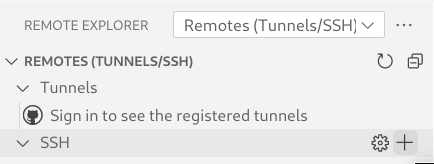
\includegraphics[frame,width=0.5\linewidth]{visual_studio_code_ssh.png}
\end{center}

\warnbox{Es recomendable hacer uso del \hyperlink{ssh_clave_publica_privada}{sistema de certificados de clave pública/privada} de SSH para realizar la conexión}

\begin{center}
    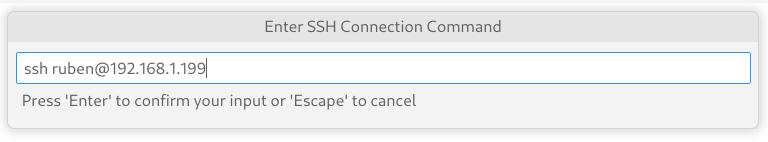
\includegraphics[width=0.9\linewidth]{visual_studio_code_ssh2.png}
\end{center}

Nos pedirá dónde queremos guardar la configuración, dejando la ruta por defecto, que es el fichero \configfile{.ssh/config} dentro de la “home” de nuestro usuario. Si hemos realizado la configuración de los certificados de clave pública/privada, no nos pedirá la contraseña.


\section{Conexión al contenedor}

Gracias a la extensión “remote development” instalada previamente, vamos a poder trabajar \textbf{dentro del contenedor de Laravel}. De esta manera Visual Studio Code va a tener acceso al intérprete de PHP para poder ayudarnos durante el desarrollo.

Hacer uso de esta funcionalidad es muy útil ya que al estar dentro del contenedor, estamos dentro del entorno de desarrollo de manera “inmersiva”, pudiendo instalar componentes o ejecutar órdenes dentro del contenedor.

Para realizar la conexión, deberemos ver los contenedores en la extensión “Remote Explorer”, en el apartado “\textbf{Dev Containers}”:

\begin{center}
    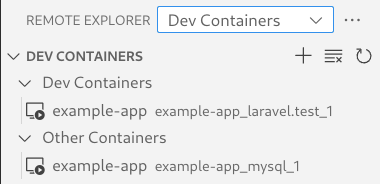
\includegraphics[frame,width=0.5\linewidth]{visual_studio_code_container.png}
\end{center}

Al acceder al contenedor, en este caso “example-app\_laravel.test\_1”, Visual Studio nos debería abrir el directorio principal donde está situada la aplicación Laravel, \configdir{/var/www/html}.